\documentclass[preview]{standalone}
\usepackage{color}
\usepackage{tikz}

% Tikz settings optimized for causal graphs.
% Copied from https://dkumor.com/posts/technical/2018/08/15/causal-tikz/
\usetikzlibrary{shapes,decorations,arrows,calc,arrows.meta,fit,positioning}
\tikzset{
    -Latex,auto,node distance =1 cm and 1 cm,semithick,
    state/.style ={circle, draw, minimum width = 1 cm},
    point/.style = {circle, draw, inner sep=0.04cm,fill,node contents={}},
    bidirected/.style={Latex-Latex,dashed},
    el/.style = {inner sep=2pt, align=left, sloped}
}
\begin{document}

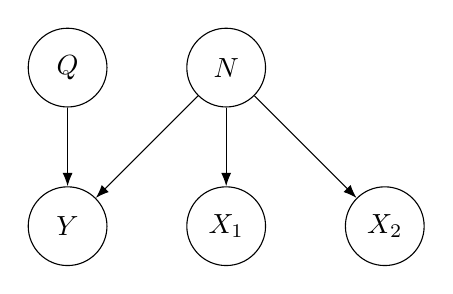
\begin{tikzpicture}
    \node[state] (q) at (0, 0) {$Q$};
    \node[state] (y) [below =of q] {$Y$};
    \node[state] (n) [right =of q] {$N$};
    \node[state] (x1) [right =of y] {$X_1$};
    \node[state] (x2) [right =of x1] {$X_2$};
    
    \path (q) edge (y);
    \path (n) edge (y);
    \path (n) edge (x1);
    \path (n) edge (x2);
\end{tikzpicture}
\end{document}